%% ----------------------------------------------------------------
%% ProjectManagement.tex
%% ---------------------------------------------------------------- 
\chapter{Project Management} 
\label{Chapter: Project Management}

\chapterpreamble{Due to the large and complex nature of the project care was taken to ensure the group's time and effort was managed effectively. This chapter gives details regarding how the group formed as well as the general positions within the team each member took. Information about the groups working procedure is given along with details of how the group communicated within itself and with project stakeholders.}

\section{Formation} 
\label{Section:Formation}

Although as a whole the group had never worked together in the past, some existing close working relationships existed due to previous group coursework. As such it was easy to form the group and begin producing impressive results.

\subsection{Skills Audit} 
\label{Section:Skills Audit}

Many of the strengths and weaknesses of the group members were clear from previous work, but a skills audit was undertaken to ensure that the group as a whole was competent to complete both the coursework and the project without fault.

To begin with a requirement analysis was performed to determine exactly what skills were needed. These split into three very clear general subsections: project management and leadership, from the perspective of both the coursework and the project; technical; and communication. 

Next an audit of each teams members skills were performed, the results of which can be found in \autoref{Chapter:Skills Audit Results}. From these an analysis of the groups total skills was determined and the groups weaknesses could be found.

\section{Task and Work Management} 
\label{Section:Task and Work Management}

This project was run using a Scrum project management approach. This involved having weekly sprints where each person completed a number of tasks, either alone or collaborating with others. Planning meetings were held at the start of each sprint where the issues in the backlog were discussed. They were prioritised and given a point value which related to how much time and effort the issue would take to resolve. The highest priority issues were then assigned. Each person had a maximum capacity of points for each week. Additionally retrospectives were held just prior to the planning meetings to discuss the previous sprints and the way in which the project management was being carried out.

This structure meant that planning and the monitoring of the project happened formally on a sprint by sprint basis. But throughout the project we were careful to adapt when needed, and not be too constrained by the Scrum model. At points in the project where progress presentations had to be created, practised and presented we ran ``mini-sprints'' both for the presentation, and work to be completed in the remainder of the week.

\todo{SCRUM roles - vauge jist of what was done and not complete}

\todo{Burndown charts and other statistics}

%http://tex.stackexchange.com/questions/86114/github-like-punchcard-with-the-help-of-pgfplots
\begin{figure}
  \makebox[\textwidth][c]{
\begin{tikzpicture}                                             %1
        \begin{axis}[                                               %2
                grid=major,                                         %3
                point meta=explicit,
                xmin=-1,
                xmax=24,
                xlabel=Hours,                                       %7
                scatter/@pre marker code/.code={
                    \pgfmathparse{                                  %12
                        sqrt(\pgfplotspointmetatransformed)/50*12}   %13
                    \def\markopts{                                  %14
                        mark=*,                                     %15
                        color=black,                     %16
                        fill=black,                      %17
                        mark size=\pgfmathresult}                   %18
                    \expandafter\scope\expandafter[\markopts]},
                scatter/@post marker code/.code={
                    \endscope},
                symbolic y coords={Sun,Sat,Fri,Thu,Wed,Tue,Mon},
                xtick={0,...,23},
                x=0.55cm,
                y=0.9cm]
            \addplot[only marks,scatter]
                table[x index=0, y index=1, meta index=2] {punchcard.dat};
        \end{axis}
\end{tikzpicture}
  }%
  \caption{Caption}
  \label{fig:key}
\end{figure}

To allow for collaborative work a GitHub organisation\footnote{\url{https://github.com/soton-ecs-2014-gdp-12/}} was used. This acted as our central source code repository for not only all directly related work, but also work on presentations and reports. Separate repositories for each area of the project are located here for ease of access. Using GitHub made it easier to interact with other open source projects, and all our pull requests and releases were directed from here. 

GitHub also provided an issue management system on a repository by repository basis. This allowed us to track conversations around different bugs and enhancements as the project progressed.
The group used \url{http://www.waffle.io} to manage the issues backlog from a project wide perspective as this would interface directly with GitHub.

%Sam has the code to generate this form the Github API
\begin{figure}
\centering
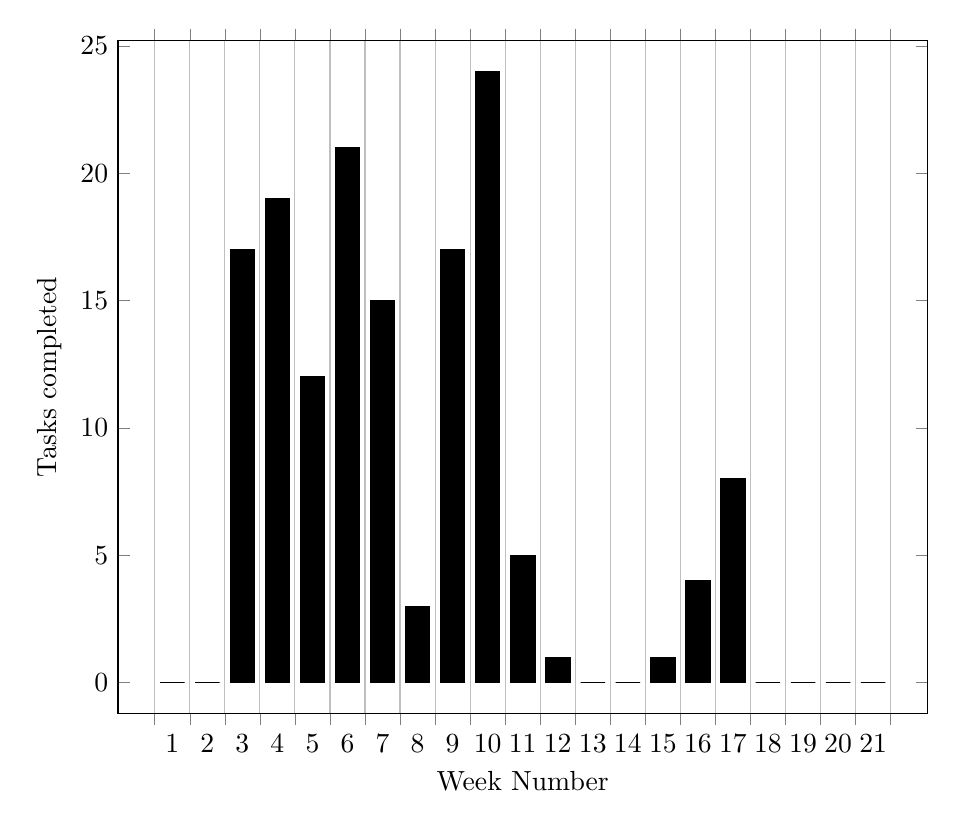
\begin{tikzpicture}
\begin{axis}[
	scale=1.5,
	ylabel={Tasks completed},
	xlabel= {Week Number},
	enlargelimits=0.05,
	ybar interval=0.7,
]
\addplot[black,fill=black]
	coordinates {(1, 0) (2, 0) (3, 17) (4, 19) (5, 12) (6, 21) (7, 15) (8, 3) (9, 17) (10, 24) (11, 5) (12, 1) (13, 0) (14, 0) (15, 1) (16, 4) (17, 8) (18, 0) (19, 0) (20, 0) (21, 0) (22, 0) };
\end{axis}
\end{tikzpicture}
  \caption{Caption}
  \label{fig:key}
\end{figure}

\section{Communication} 
\label{Section:Communication}

The project had a reasonably large number of stakeholders that needed to be managed and kept informed. Each stakeholder required different levels of communication via different methods.

The most important stakeholder was the client, Professor Mike Wald. Weekly meeting were organised, minutes of which can be found in Appendix BLAH, and emails were used for urgent issues. 
\todo{Appendix of minutes}
\todo{Managing client - signoff, etc}
Another important stakeholder was Yunjia Li. He attend the weekly meetings as much as possible so as to ensure his future interests in the framework were protected. He was also contactable via email when needed.

2fdev, the Videogular development team, were communicated with via Gitter\footnote{\url{https://gitter.im/2fdevs/videogular}}, an online chat system added onto GitHub. They had an ongoing interest with the framework due to its role of advertising the Videogular project.  There advice and code proved invaluable throughout the project.

\todo{Shameem stakeholder/team member/client discuss}



